\usetikzlibrary{arrows,positioning}
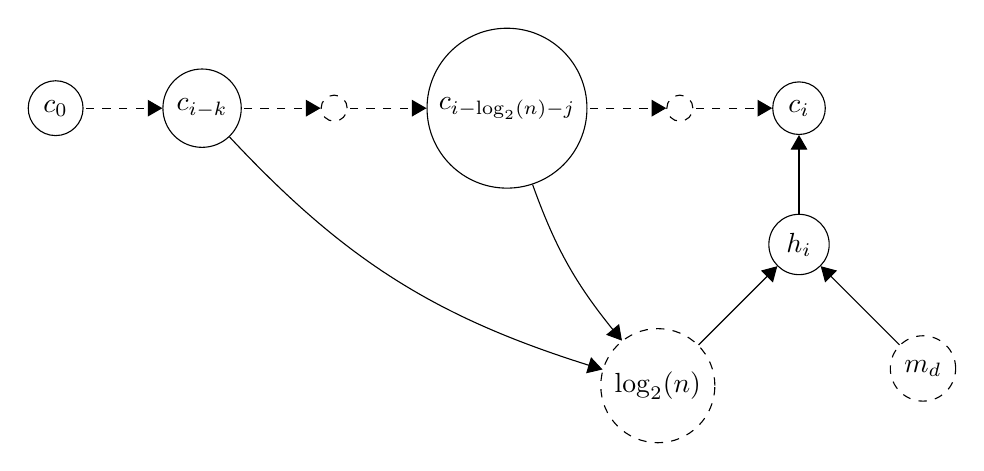
\begin{tikzpicture}[every node/.style={circle,draw},
                                    every path/.style={<-,>=triangle 60}]

\node (c0) {$c_0$};
\node[right=of c0] (ck) {$c_{i-k}$} edge[dashed] (c0);
\node[right=of ck,dashed] (ckmiddle) {} edge[dashed] (ck);
\node[right=of ckmiddle] (ci2){$c_{i-\log_2(n)-j}$} edge[dashed] (ckmiddle);
\node[right=of ci2,dashed] (ci2middle) {} edge[dashed] (ci2);
\node[right=of ci2middle] (ci) {$c_i$} edge[dashed] (ci2middle);

\node[below=of ci] (hi) {$h_i$} edge[->] (ci);
\node[below right=of hi,dashed] (md) {$m_d$} edge[->] (hi);
\node[below left=of hi,dashed] (ms) {$\log_2(n)$} edge[->] (hi) edge[<-,bend left=10] (ci2) edge[<-,bend left=15] (ck);

\end{tikzpicture}